\documentclass[]{report}
\usepackage{graphicx, float}
\usepackage[export]{adjustbox}

\title{\centering CSP334 : Computer Networks \\Lab Assignment No 2\\Assignment on Linux Networking Commands}
\author{\LARGE Sahil\\2016UCS0008}

% to use proper section numbering in the report type 
\renewcommand{\thesection}{\arabic{section}}

\begin{document}

\maketitle

%%%%%%%%%%%%%%%%%%%%%%%%%%%%%%%%%%%%%%%%%%%%%%%%
\section{Problem 1:}

\subsection{/etc/hosts} 
\begin{figure}[H]
	\vspace{0pt}
	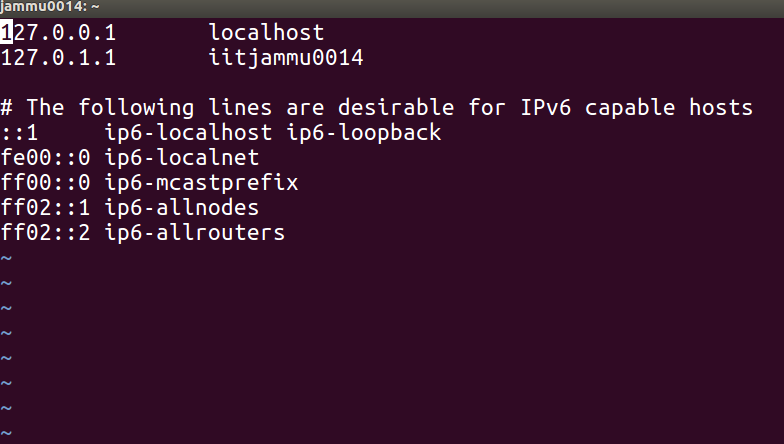
\includegraphics[width=\linewidth, keepaspectratio]{Snapshots/exe1/hosts.png}
\end{figure}
It is used to bypass DNS resolution. Any match found in it will be used before DNS entry. It can be used to given human readable names to some local machines on a small network.
 
\subsection{/etc/sysconfig/network}
This file stores the host name and default gateway IP address.

\subsection{/etc/sysconfig/network-scripts/ifcfg-eth0}
This stores the IP address of the first ethernet interface.

\subsection{/etc/default-route}
This stores a default gateway i.e. the IP address/domain name of the default router.

\subsection{/etc/resolv.conf}
\begin{figure}[H]
	\vspace{0pt}
	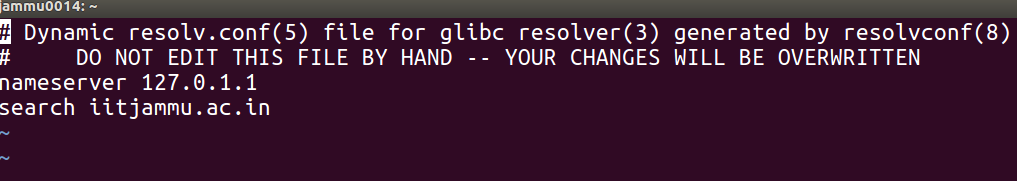
\includegraphics[width=\linewidth, keepaspectratio]{Snapshots/exe1/resolv_conf.png}
\end{figure}
It is used to store the information about the paramters of the DNS resolver which allows the system to translate human friendly domain names into IP addresses.

\subsection{/etc/nsswitch.conf}
\begin{figure}[H]
	\vspace{0pt}
	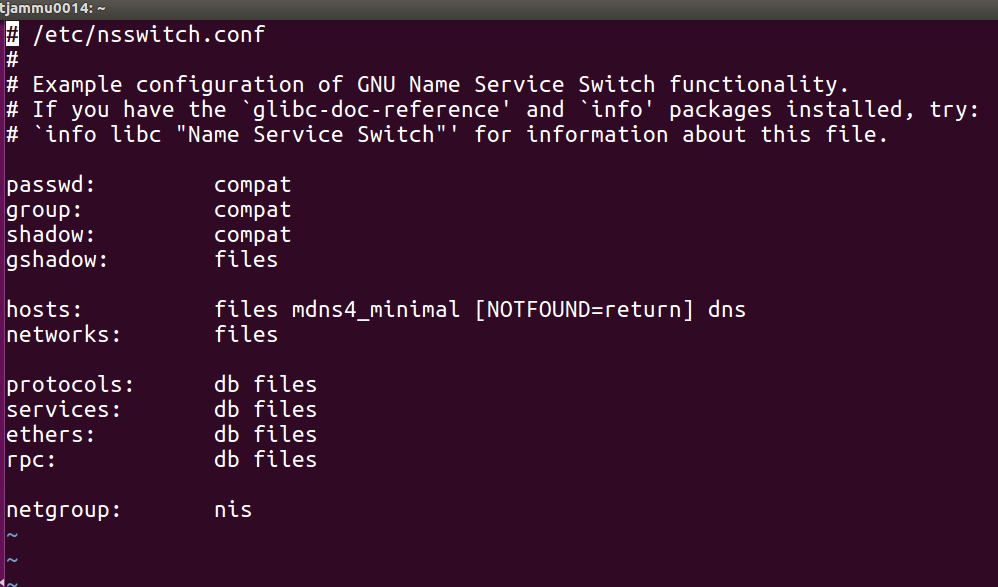
\includegraphics[width=\linewidth, keepaspectratio]{Snapshots/exe1/nsswitch.png}
\end{figure}
It is used to specify the order of name resolution, for e.g.\textbf{hosts: files dns} means that first check in files and if not found, then try DNS. 


%%%%%%%%%%%%%%%%%%%%%%%%%%%%%%%%%%%%%%%%%%%%%%%%
\section{Problem 2: /etc/services}
\begin{figure}[H]
	\vspace{0pt}
	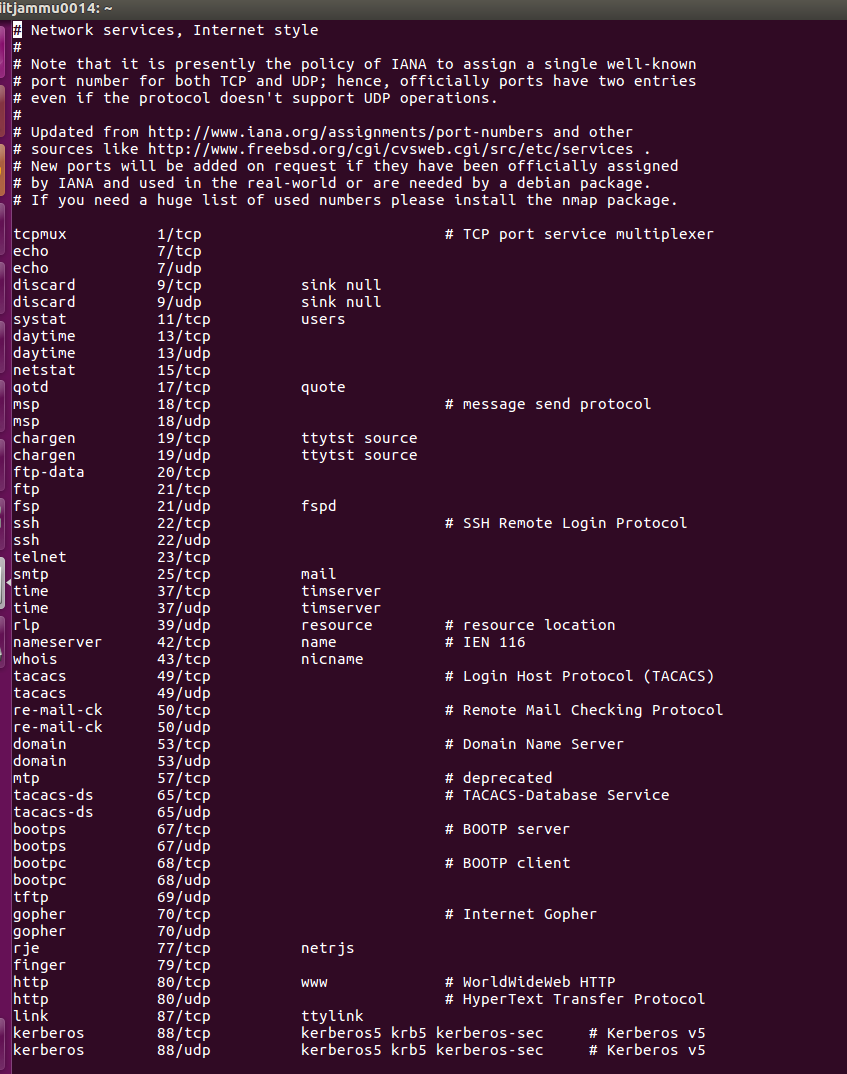
\includegraphics[width=\linewidth, keepaspectratio]{Snapshots/exe2/services.png}
\end{figure}

\subsection{Use}
This file provides the details of the port no. associated with a service and thus when the packet is sent from the local machine, the port no. is attached from this file. 

\subsection{Layer}
It uses the transport layer as that provides process-to-process message delivery.

\subsection{Port numbers}
The port numbers shown are ONLY \textbf{well-known} port numbers. This is because we must know the port number on the remote machine before sending a request using transport layer, so they are recognized through this file. 

%%%%%%%%%%%%%%%%%%%%%%%%%%%%%%%%%%%%%%%%%%%%%%%%
\section{Problem 3: Basic linux commands}
\large
\begin{center}
	\begin{tabular}{ |p{1cm}|p{1.4cm}||p{5cm}|p{1.0cm}|p{1.0cm}|p{1.2cm}||  }
		\hline
		S.No & Name	&	Purpose	&	App. Layer Protocol	&	Trans - port Layer Protocol	&	Network Layer Protocol	\\
		\hline
		1 & arp         & It is used to convert the IP address to the Physical address or the MAC address. & - & - & -						\\
		2 & arping    & It is used to send ARP requests to a machine on local network. In response, we get the physical address of the machine. & - & - & ARP				\\
		3 & ifconfig  & It basically tells about the network interfaces and the assigned IP address to the local machine. & - & - & -						\\
		4 & tcpdump& It is used to capture packets on a network interface and the type of packets to be captured can be defined on the protocol or IP addresses associated. & - & - & -						\\
		5 & ping       & It is used to test the ability of the source computer to reach a specified destination computer. It sends ICMP request messages to the destination computer. & - & ICMP & IP						\\
		6 & netstat   & It is used to display routing tables, active TCP connections and some other network protocol stats. & - & - & -						\\
		7 & route      & It is used to modify the network routing tables. & - & - & -						\\
		\hline
	\end{tabular} 
\end{center}

%%%%%%%%%%%%%%%%%%%%%%%%%%%%%%%%%%%%%%%%%%%%%%%%
\section{Problem 4: Capturing tcpdump traffic}
\begin{figure}[H]
	\vspace{0pt}
	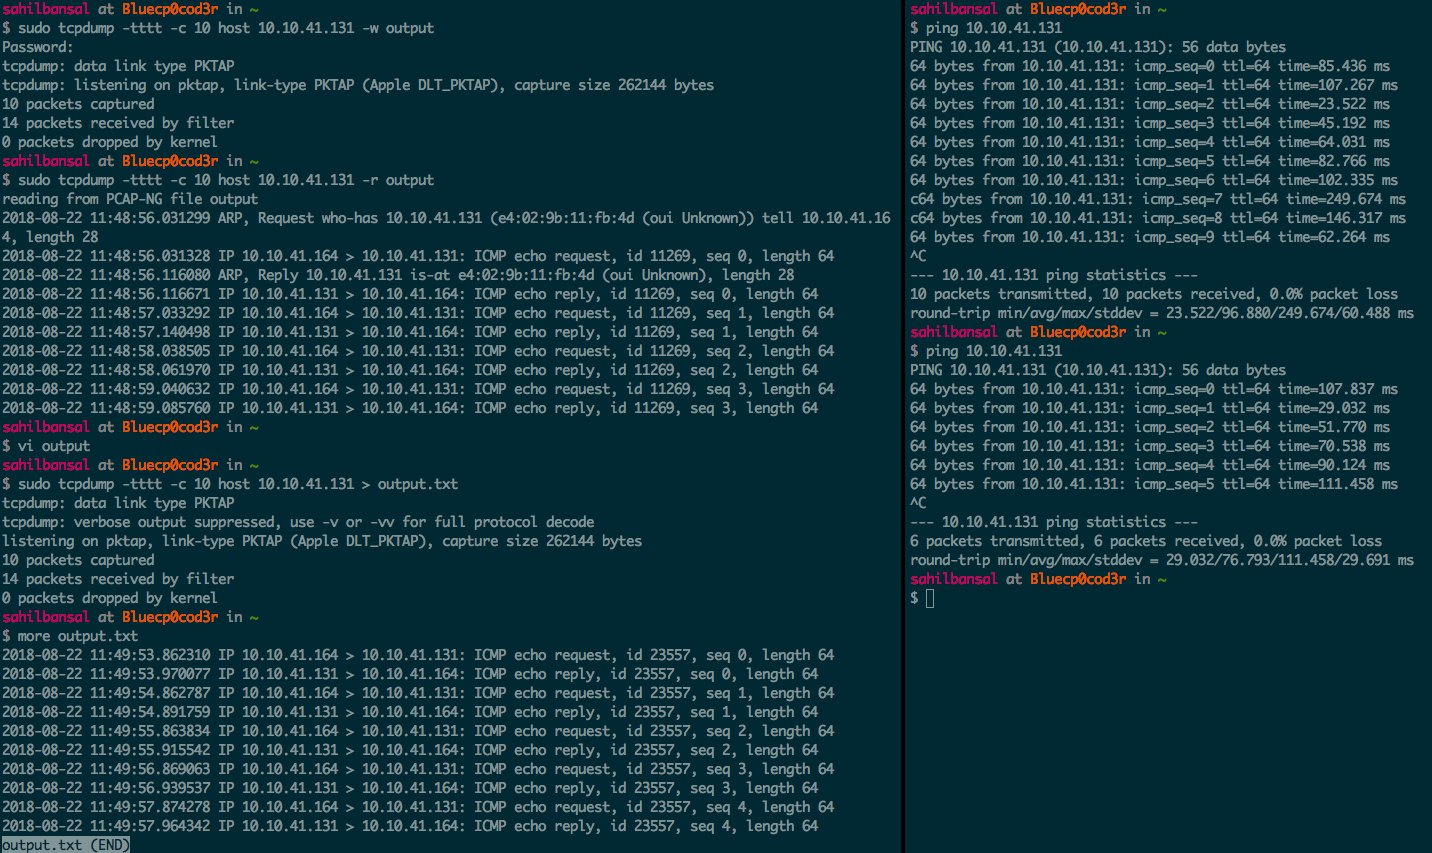
\includegraphics[height=500pt, width=600pt, center]{Snapshots/exe4/tcpdump.png}
\end{figure}
The options used for the tcpdump command are -tttt, to display a better time format, -c 10, to restrict the no. of packets captured to 10, and the output is redirected to a text file using $>$ command. If we use -w option, then the file would contain data in unreadable format, which can only be recognized using -r option or using wireshark. 

%%%%%%%%%%%%%%%%%%%%%%%%%%%%%%%%%%%%%%%%%%%%%%%%
\section{Problem 5: tcpdump -enx -w exe5.out}
\begin{figure}[H]
	\vspace{0pt}
	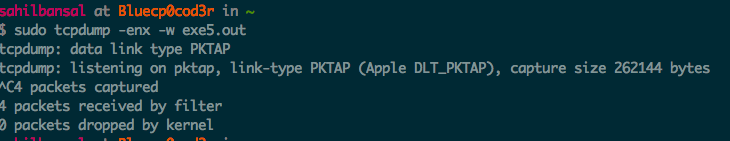
\includegraphics[width=600pt, keepaspectratio, center]{Snapshots/exe5/tcpdump_w.png}
\end{figure}

The above command captures the packets in the file named \textbf{exe5.out} from the \textbf{ethernet (enx)} interface, because \textbf{-w} option is used. Thus, the details of packets captured is not output on the screen. Although, it shows the statistics at the end, i.e.:
\begin{itemize}
	\item No. of packets captured
	\item No. of packets received by filter
	\item No. of packets dropped by kernel
\end{itemize}

%%%%%%%%%%%%%%%%%%%%%%%%%%%%%%%%%%%%%%%%%%%%%%%%
\section{Problem 6: Capture packets generated using telnet utility}
\begin{figure}[H]
	\vspace{0pt}
	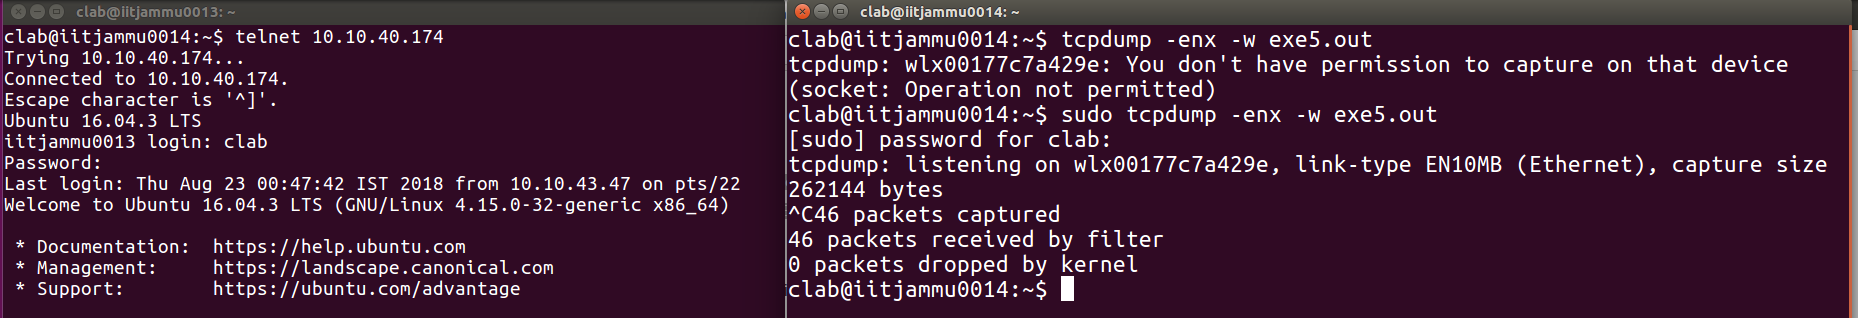
\includegraphics[width=600pt, keepaspectratio, center]{Snapshots/exe6/telnet.png}
\end{figure}

\subsection{Format of the packet saved:}
\subsubsection{Link Header: }
\begin{figure}[H]
	\vspace{0pt}
	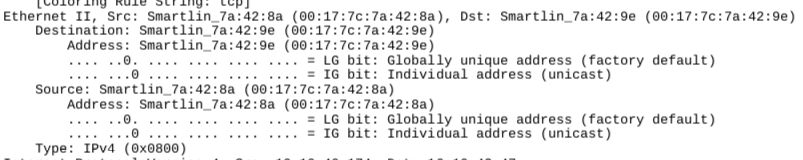
\includegraphics[width=600pt, keepaspectratio, center]{Snapshots/exe6/eth.png}
\end{figure}
\begin{tabular}{ |p{4cm}|p{4cm}|p{4cm}| }
	\hline
	Destination Address: 00:17:7c:7a:42:9e & Source Address: 00:17:7c:7a:42:8a & Frame Type: IPv4 (0x0800) \\
	\hline
\end{tabular}

\subsubsection{IP Header: }
\begin{figure}[H]
	\vspace{0pt}
	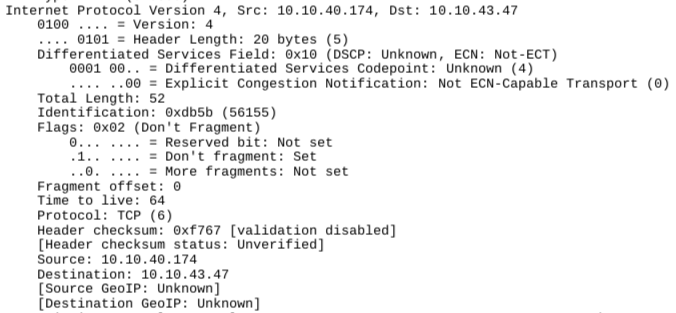
\includegraphics[width=600pt, keepaspectratio, center]{Snapshots/exe6/ip.png}
\end{figure}
\begin{tabular}{ |p{3cm}|p{3cm}|p{3cm}|p{3cm}|  }
	\hline
	Version: 4 & Header Length: 20 & Differentiated Services: 16  & Total length: 52 \\
	\hline
	\multicolumn{2}{|c|}{Identification: 56155} & Flags: 2 & Fragment Offset: 0 \\
	\hline
	Time to live: 64 & Protocol: TCP & \multicolumn{2}{|c|}{Header Checksum: 63335} \\
	\hline
	\multicolumn{4}{|c|}{Source IPA: 10.10.40.174} \\
	\hline
	\multicolumn{4}{|c|}{Destination IPA: 10.10.43.47} \\
	\hline 
\end{tabular}

\subsubsection{TCP Header: }
\begin{figure}[H]
	\vspace{0pt}
	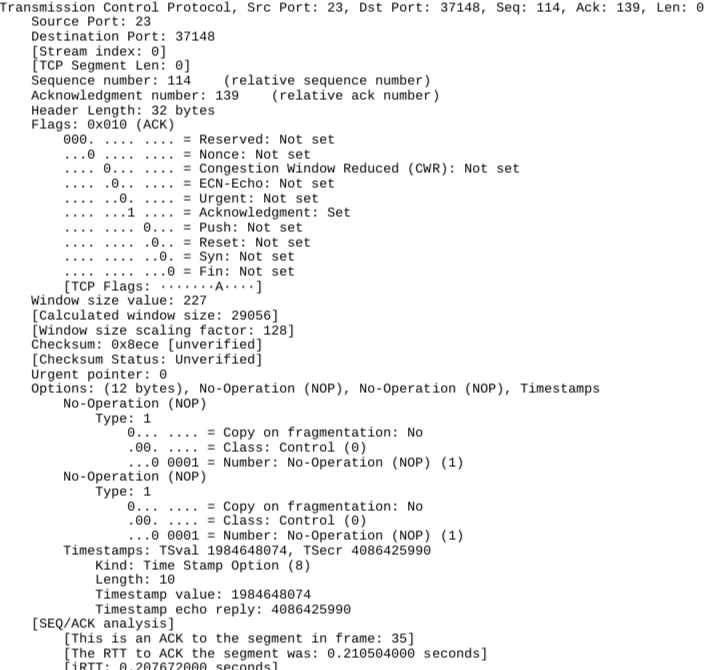
\includegraphics[height=400pt, keepaspectratio, center]{Snapshots/exe6/tcp.png}
\end{figure}
\begin{tabular}{ |p{3cm}|p{3cm}|p{3cm}|p{3cm}|  }
	\hline
	\multicolumn{2}{|c|}{Source Port No: 23} & \multicolumn{2}{|c|}{Destination Port No: 37148} \\
	\hline
	\multicolumn{4}{|c|}{Sequence Number: 114 (relative)} \\
	\hline
	\multicolumn{4}{|c|}{Acknowledgement Number: 139 (relative)} \\
	\hline 
	Header Length: 32 & Reserved & Flags: 16 & Window Size: 227 \\
	\hline
	\multicolumn{2}{|c|}{TCP Checksum: 36558} & \multicolumn{2}{|c|}{Urgent Pointer: 0} \\
	\hline
	\multicolumn{4}{|c|}{Options: 12 bytes} \\
	\hline
\end{tabular}

\subsection{Protocol field in the IP header of the packet: }
The value in this field is \textbf{TCP} and it tells which protocol will be used in the above layer as network layer forwards the packet to transport layer at the destination. In other words, it specifies the transport-layer protocol encapsulated by the datagram.

%%%%%%%%%%%%%%%%%%%%%%%%%%%%%%%%%%%%%%%%%%%%%%%%
\section{Problem 7: Capture ARP requests and replies using tcpdump}
\begin{figure}[H]
	\vspace{0pt}
	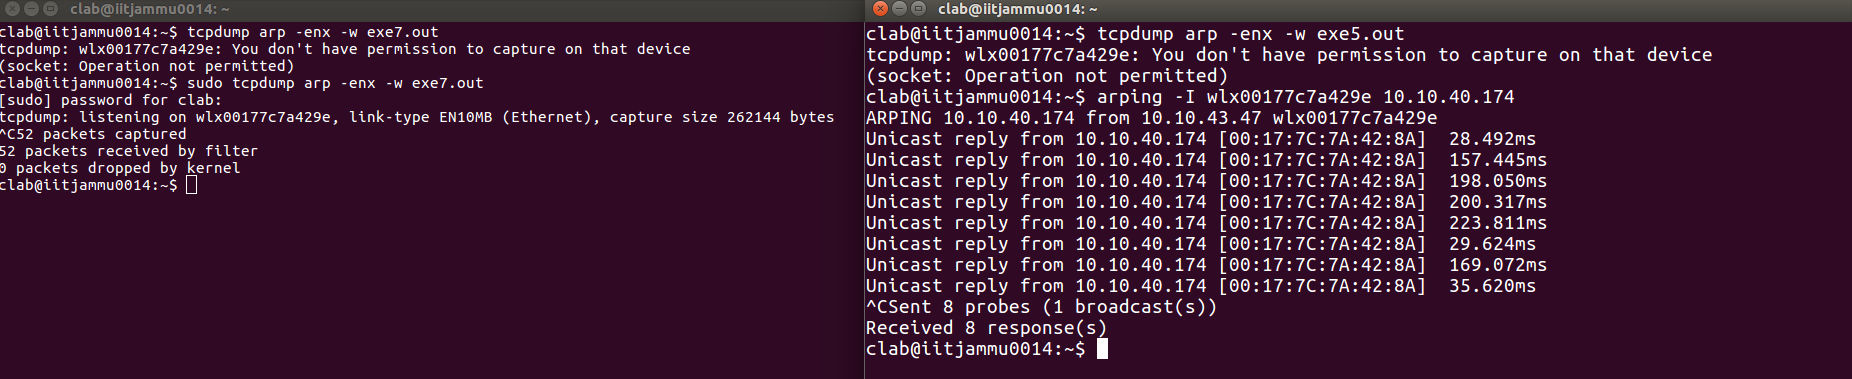
\includegraphics[width=600pt, keepaspectratio, center]{Snapshots/exe7/arping.png}
\end{figure}

\begin{figure}[H]
	\vspace{0pt}
	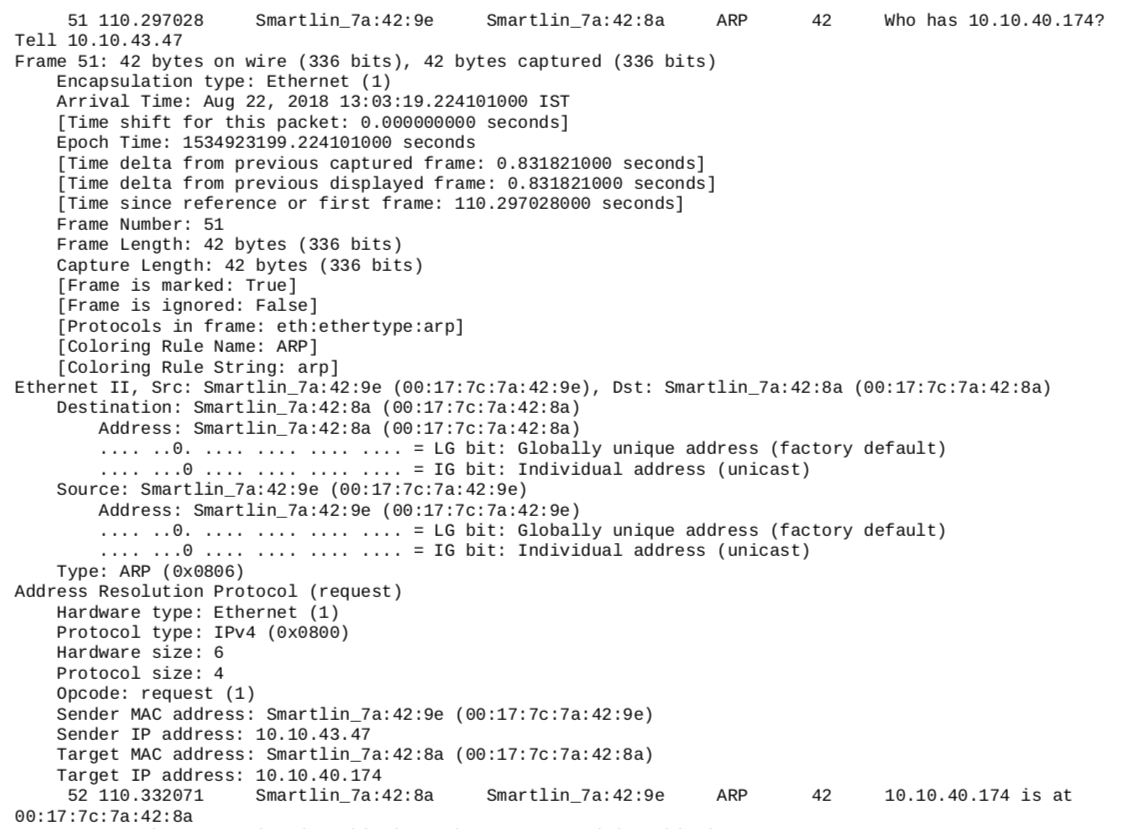
\includegraphics[height=400pt, keepaspectratio, center]{Snapshots/exe7/req.png}
\end{figure}

\begin{figure}[H]
	\vspace{0pt}
	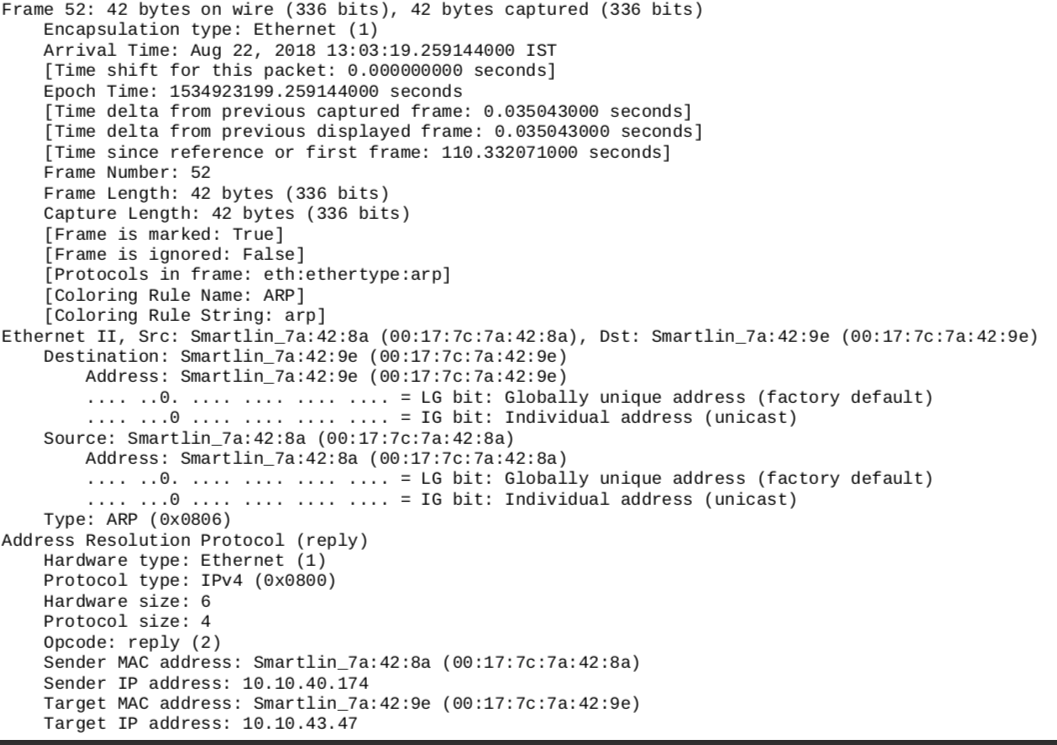
\includegraphics[height=400pt, keepaspectratio, center]{Snapshots/exe7/rep.png}
\end{figure}

\subsection{Frame type field in an Ethernet frame carrying an ARP request and ARP reply: }
This value is \textbf{ARP (0x0806)} in both the request and the reply.

\subsection{Frame type field in an Ethernet frame carrying an IP datagram in previous exercise: }
This value is \textbf{IPv4 (0x0800)}.

\subsection{Use of frame type field: }
This tells which protocol is to be used in the network layer, i.e. provides the information about the type of the payload. 

%%%%%%%%%%%%%%%%%%%%%%%%%%%%%%%%%%%%%%%%%%%%%%%%
\section{Problem 8: Some tcpdump expressions and their meanings}

\subsection{tcpdump udp port 520}
It captures UDP packets on port no. 520. 

\subsection{tcpdump -x -s 120 ip proto 89}
The -x option is used to print the data in hex and the -s option defines the snaplength, i.e. the maximum bytes of data which can be captured for a packet. Here, the size is 120 bytes. The \textbf{ip proto 89} option restricts the capture of only the protocol having no. 89, i.e. OSPF (Open Shortest Path First). 

\subsection{tcpdump -x -s 70 host ip addr1 and (ip addr2 or ip addr3)}
It captures those packets which involve communication between ip address 1 and either of the ip address 2 or the ip address 3.
\begin{figure}[H]
	\vspace{0pt}
	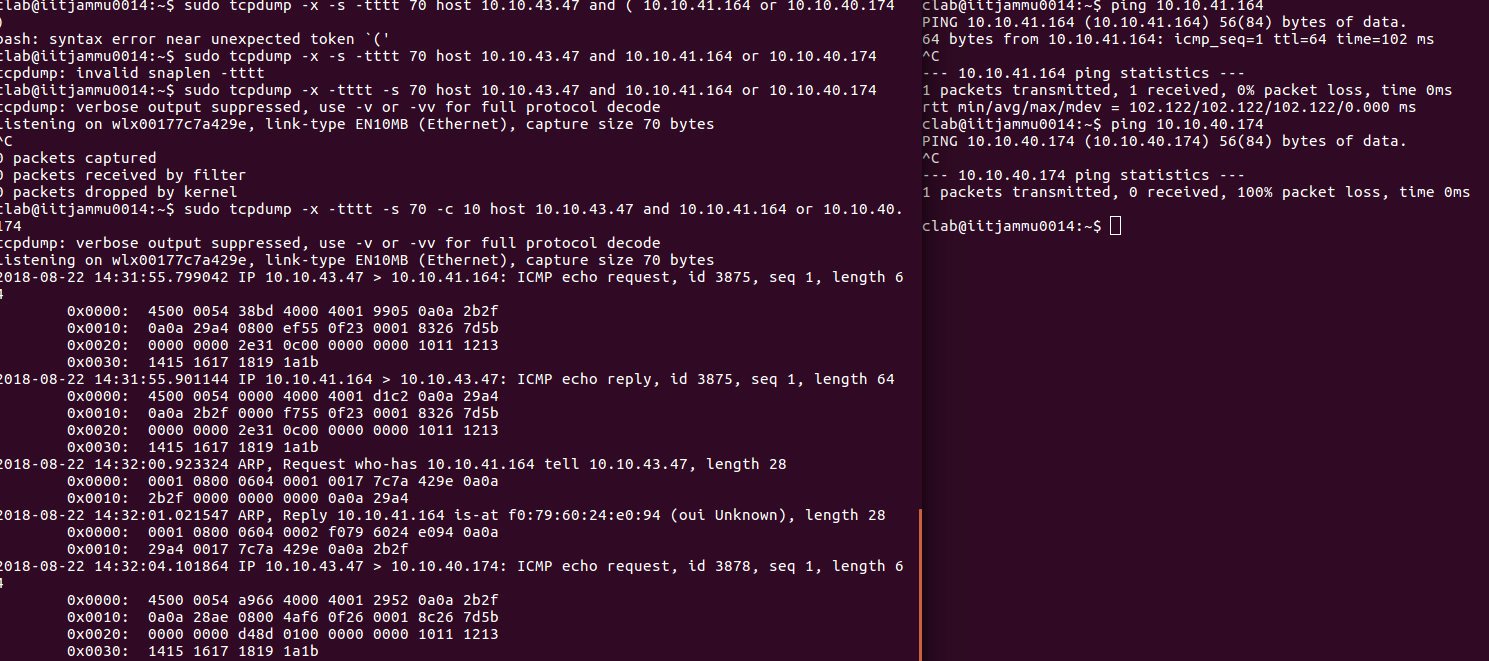
\includegraphics[width=600pt, keepaspectratio, center]{Snapshots/exe8/q8_3.png}
\end{figure} 

\subsection{tcpdump -x -s 70 host ip addr1 and not ip addr2}
It used to capture those packets which involve ip address 1 but do not involve ip address 2. 
\begin{figure}[H]
	\vspace{0pt}
	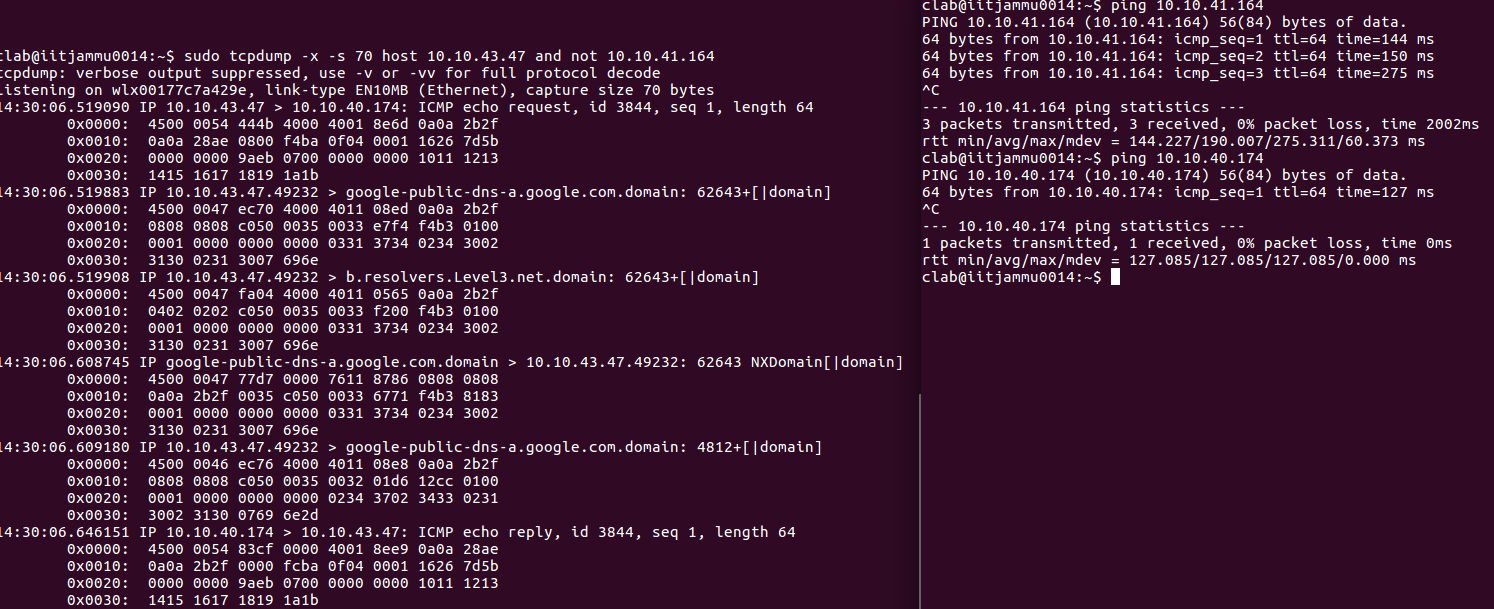
\includegraphics[width=600pt, keepaspectratio, center]{Snapshots/exe8/q8_4.png}
\end{figure} 
%%%%%%%%%%%%%%%%%%%%%%%%%%%%%%%%%%%%%%%%%%%%%%%%
\section{Problem 9: Analyze port numbers in telnet communication}
\begin{figure}[H]
	\vspace{0pt}
	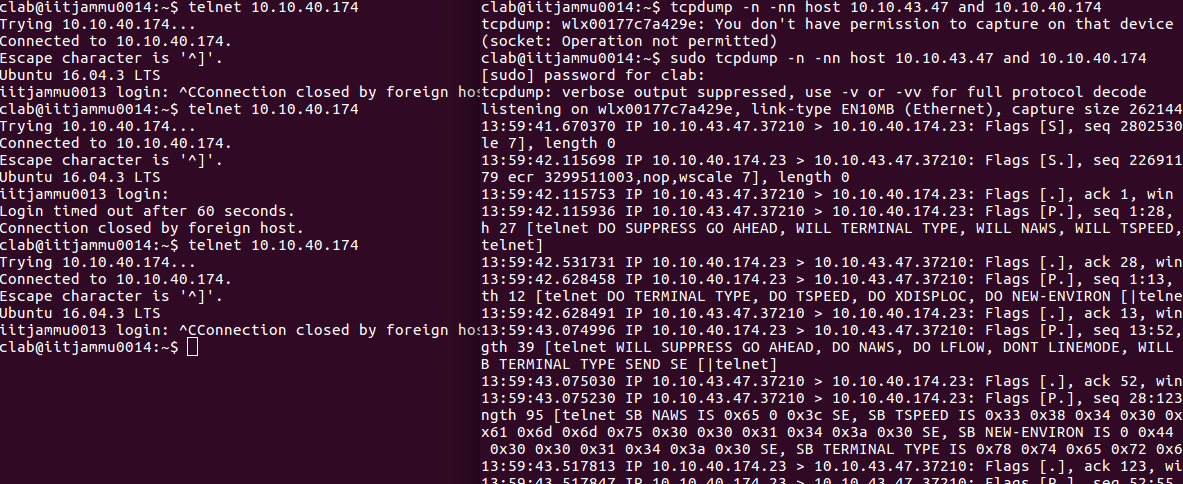
\includegraphics[width=600pt, keepaspectratio, center]{Snapshots/exe9/q9.png}
\end{figure} 
\begin{figure}[H]
	\vspace{0pt}
	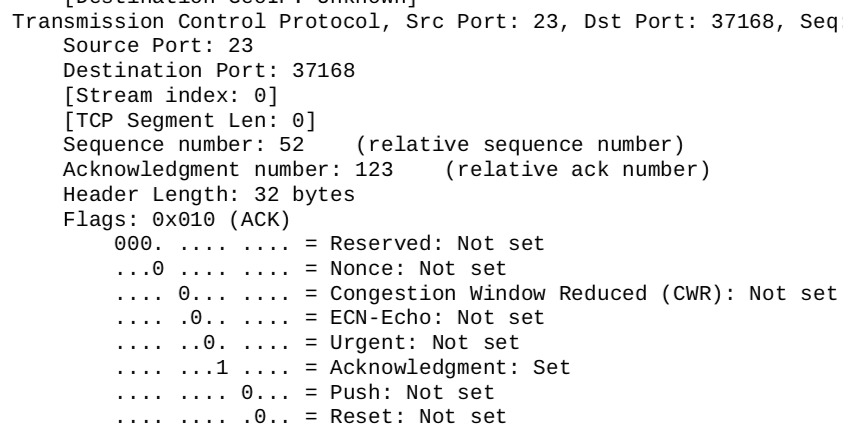
\includegraphics[width=600pt, keepaspectratio, center]{Snapshots/exe9/ports.png}
\end{figure} 
\subsection{Port numbers used: }
The port no. used by the local machine is 37168 and that by the remote machine is 23.
\subsection{Port number matching the one for telnet: }
That of the \textbf{remote} machine matches to the port no. of telnet (23). This is because it acts like a server and must use a well-known port number for the TCP communication. 

%%%%%%%%%%%%%%%%%%%%%%%%%%%%%%%%%%%%%%%%%%%%%%%%
\section{Problem 10: Analyzing port numbers when two telnet sessions open simultaneously}
\begin{figure}[H]
	\vspace{0pt}
	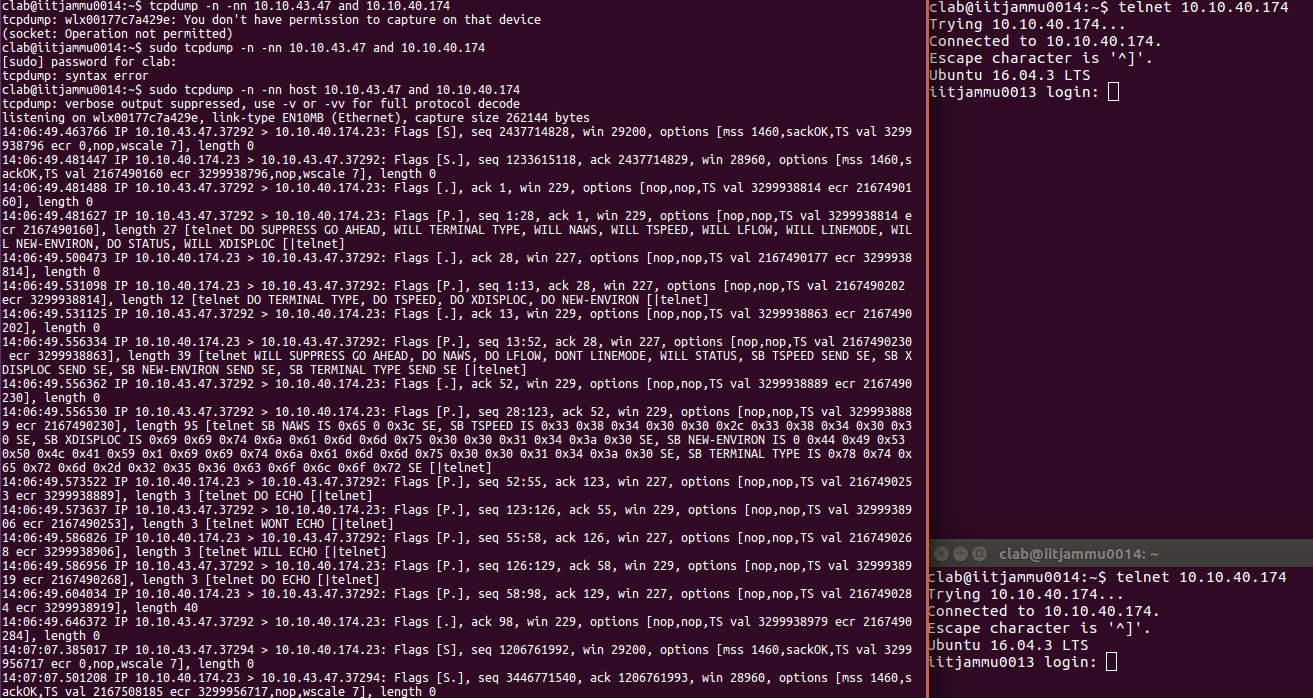
\includegraphics[width=600pt, keepaspectratio, center]{Snapshots/exe10/q10.png}
\end{figure} 
\begin{figure}[H]
	\vspace{0pt}
	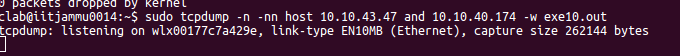
\includegraphics[width=600pt, keepaspectratio, center]{Snapshots/exe10/q10_2.png}
\end{figure} 

\begin{figure}[H]
	\vspace{0pt}
	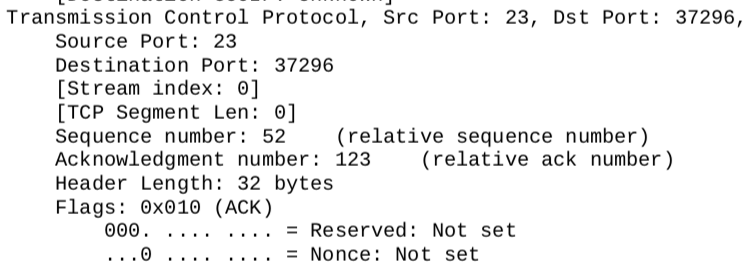
\includegraphics[width=600pt, keepaspectratio, center]{Snapshots/exe10/session1.png}
\end{figure} 
\begin{figure}[H]
	\vspace{0pt}
	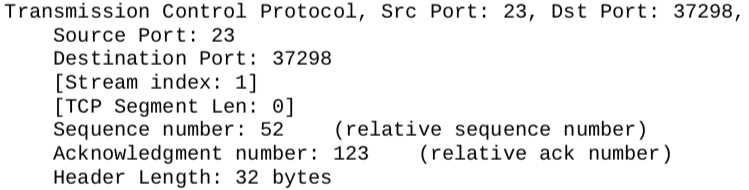
\includegraphics[width=600pt, keepaspectratio, center]{Snapshots/exe10/session2.png}
\end{figure} 

\subsection{Port number used on the remote machine: }
Port number 23 is used on the remote machine, which is the same for both the sessions.

\subsection{Port number used on the local machine: }
The port numbers used on the local machine for both the sessions are different and are 37296 \& 37298. 

\subsection{Well-known port numbers and consistency: }
\begin{itemize}
	\item The range of internet-wide well-known port no is from 0 to 1023.
	\item The range of well-known port numbers for Unix/Linux specific service is from 0 to 1023. 
	\item The range for a client port number is from 1024 to 65535.
	\item \textbf{Consistency:} It is not consistent with the well-known port numbers given in the /etc/services file, since this file also contains ports above no. 1024 which are still considered well-known in the file. This is because most of them are not running on the server, and thus the client can use those ports.
\end{itemize} 
\end{document}
